% Nastavení dokumentu

\documentclass[FM,DP]{tulthesis}  % Diplomová práce fakulty mechatroniky
\usepackage[czech]{babel}  % Česká šablona dokumentu
\usepackage[utf8]{inputenc}  % Česká diakritika
\usepackage{graphicx}  % Tvorba tabulek
\usepackage{float}  % Ukotvení věcí na svém místě (obrázky, tabulky, grafy, ...)
\usepackage{hyperref}  % Klikací odkazy v obsahu a referencích
\usepackage{gensymb}  % Pro stupne celsia
\usepackage{url}  % Pro lomeni adres url

% Titulní stránka

\TULtitle{Inteligentní domovní systém}{Smart home system}
\TULprogramme{N2610}{Elektrotechnika a informatika}{Electrical Engineering and Informatics}
\TULbranch{1802T007}{Informační technologie}{Information Technology}
\TULauthor{Bc. Tomáš Moravec}
\TULsupervisor{doc. Ing. Josef Chaloupka, Ph.D.}
\TULyear{2018}

% Prohlášení

\begin{document}
\ThesisStart{male}

% Poděkování

\begin{acknowledgement}
Děkuji vedoucímu práce panu doc. Ing. Josefu Chaloupkovy, Ph.D. za odborné vedení a poskytnuté informace při zpracování závěrečné diplomové práce.
\end{acknowledgement}

% Abstrakt

\begin{abstractCZ}
Práce se zabývá vytvořením inteligentního domovního systému, určenému ke zpracování dat z bezpečnostních a meteorologických čidel, a řízení vybraných domovních zařízení. Komplexní řešení zahrnuje jak samotný domovní systém, tak mobilní, webovou a desktopovou aplikaci. V úvodu jsou definovány základní pojmy a požadované vlastnosti. Následuje rešerše a výběr vhodných hardwarových a softwarových řešení. Ná základě rešerše je navržen koncept komplexního domovního systému, který je následně realizován v jednotlivých etapách. Výstupem práce je funkční cílové zařízení, které aplikuje zvolené hardwarové i softwarové řešení.

\end{abstractCZ}

\vspace{2cm}

\begin{abstractEN}
Not implemented yet.
\end{abstractEN}

% Seznam zkratek

\tableofcontents
\clearpage

\begin{abbrList}
\textbf{API} & Application Programming Interface, rozhraní pro přístup k aplikaci\\
\textbf{GBS} & Glass break detector, detektor rozbití skla\\
\textbf{GPRS} & General Packet Radio Service, služba pro přenos dat v mobilní síti\\
\textbf{GSM} & Groupe Spécial Mobile, globální systém pro mobilní komunikaci\\
\textbf{GUI} & Graphical User Interface, grafické uživatelské rozhraní\\
\textbf{IDE} & Integrated development environment, integrované vývojové prostředí\\
\textbf{LAN} & Local Area Network, místní počítačová síť\\
\textbf{LED} & Light-Emitting Diode, dioda emitující světlo\\
\textbf{PIR} & Passive infrared sensor, infračervený sensor pohybu\\
\textbf{SMS} & Short message service, služba krátkých textových zpráv\\
\textbf{TUL} & Technical University of Liberec, Technická univerzita v Liberci\\
\textbf{USB} & Universal Serial Bus, univerzální sériová sběrnice\\

\end{abbrList}

% Úvod

\chapter{Úvod}
Not implemented yet.

% Zabezpečovací systém
\chapter{Zabezpečovací systém}
Zabezpečovací systém, někdy také elektronická zabezpečovací signalizace, je zařízení, které vizuálně nebo akusticky vyhlašuje poplach a dává na vědomí, že nastaly nějaké potíže nebo došlo ke splnění sledované podmínky \cite{Security alarm}. Jde tedy o zařízení, které slouží k ochraně osob a majetku. Systém je řízen ústřednou a může se spustit analogovou (např. dveřní, či okenní čidlo) i digitální (detektor pohybu) detekcí. Komunikace mezi detektory a ústřednou může být vedena kabelem, bezdrátově anebo kombinací předešlých způsobů, tj. jeden detektor může být připojen kabelem a druhý bezdrátově \cite{Electronic security system}.

\section{Ústředna}
Ústředna je „mozek“ celého systému, který je propojen s ostatními prvky systému kabely nebo bezdrátově. Obstarává komunikaci mezi jednotlivými komponenty systému, má v integrované paměti uložené nejdůležitější nastavení \cite{Electronic security system}. V závislosti na připojených komponentech pak může různě reagovat na splnění sledovaných podmínek. Často bývá vybavena jenom tím nejnutnějším pro vyvolání poplachu, to ať už akustického (siréna), nebo tichého (informování majitele) \cite{Security alarm}.

\section{Ovladač}
Ovladač je prvek, který slouží k ovládání a případně též k programování ústředny. Dnešní alarmy je možné ovládat několika způsoby. Jako ovladač se nejčastěji používá klávesnice vybavená tlačítky, případně čtečkou (čipovými kartami a přívěšky) nebo též dálkové ovládání. U některých systémů se dá přes klávesnici provést nastavení celého systému. Klávesnice slouží k zastřežení i odstřežení systému \cite{Electronic security signalisation}. Dalšími způsoby je ovládání přes internet, kdy se většinou používá integrované webové rozhraní, ke kterému se uživatel může připojit po zadání hesla, nebo ovládání přes mobil (SMS příkazy) \cite{Bachelor thesis}.

\section{Detektor}
Detektor je prvek systému, který je rozmístěn v hlídaném objektu a má za úkol reagovat aktivací při narušení (otevření, pohyb, rozbití atd.) a to tak, že tuto informaci předají ústředně, která ji následně zpracuje \cite{Electronic security signalisation}. Nejčastěji používané detektorové prvky jsou:

\begin{itemize}
\item Magnetický kontakt (dveřní čidlo)
\item Detektor pohybu (PIR detektor)
\item Detektor tříštění skla (GBS detektor)
\item Detektor plynu
\item Infra závora
\end{itemize} 

\section{Komunikátor}
Komunikátor je zařízení, které odesílá informaci o narušení objektu, případně o odchylce od normálního provozního stavu zabezpečovacího systému \cite{Electronic security signalisation}. Nejčastější typy komunikátorů jsou:

\begin{itemize}
\item GSM komunikátor
\item LAN komunikátor
\item Telefonní komunikátor
\item Komunikátor využívající radiové sítě s vyhrazenou frekvencí
\end{itemize} 

% Požadované vlastnosti a zvolené komponenty

\chapter{Požadované vlastnosti a zvolené komponenty}
V následující části se zaměřím na požadované vlastnosti zabezpečovacího zařízení, a jaké komponenty byly na jejich základě zvoleny.

\section{Hardware}
Z úvodní části je zřejmé, že kompletní zabezpečovací systém musí obsahovat detektory, komunikátor a ústřednu. Rozebereme si tedy jednotlivé části.

\subsection{Ústředna}
Požadavky na ústřednu jsou takové, že musí být schopná komunikovat jak s desktopovou aplikací, tak s mobilní aplikací a zároveň musí řídit a zpracovávat jednotlivé komponenty. Již ze zadání diplomové je zřejmé, že ústřednou bude vývojová platforma Arduino \cite{Pruvodce arduinem}, která je se svými periferiemi \cite{Arduino schematic} a čipem Atmega \cite{Atmega datasheet}, více než vhodnou pro tyto účely. Firmware ústředny bude psán v jazyku  C++ s nadstavbou Wiring (knihovna pro řízení hardwaru) \cite{Wiring} a vývoj bude probíhat v prostředí Visual Studio 2017 s rozšířením Visual Micro \cite{Visual Micro}, které poskytuje zvýrazňování syntaxe knihovny Wiring a umožňuje komplikaci a nahrávání kódu přímo na desku Arduino.

\paragraph{Zvolená ústředna:}
\begin{itemize}
\item Arduino Uno Rev3 (700 Kč s DPH), (\url{arduino-shop.cz})
\end{itemize}

\begin{figure}[H]
\begin{center}
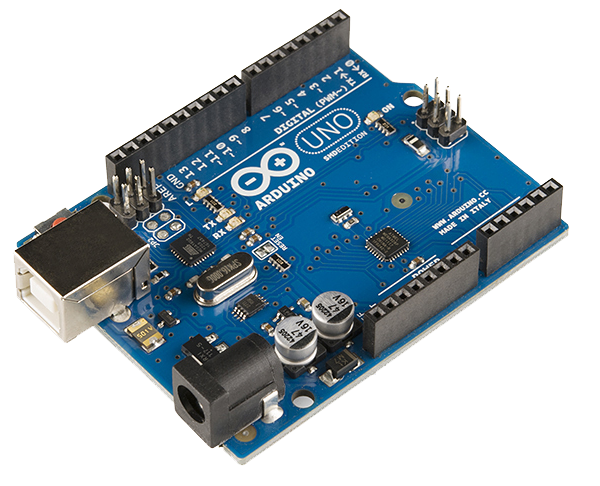
\includegraphics[width=0.4\textwidth]{images/arduino.png}
\caption{Vývojová platforma Arduino}
\label{image}
\end{center}
\end{figure}

\subsection{Detektory}
Požadavky nejsou kladeny pouze na samotné detektory, ale také na spínače, kterými bude možné spínat různá zařízení. Jako spínací prvky není nutné volit jednotlivé komponenty, stačí připravit implementaci jejich spínání. V případě detektorů musí být možné připojit libovolný detektor, který lze nastavit jako spínací (normálně rozepnutý), nebo rozpínací (normálně sepnutý). Pro testovací účely byly zvoleny dva detektory, každý jednoho typu.

\paragraph{Zvolené detektory:}
\begin{itemize}
\item Dveřní čidlo (rozpínací), (poskytl vedoucí)
\item PIR detektor (spínací), (25 Kč s DPH), (\url{aliexpress.com})
\end{itemize} 

\begin{figure}[H]
\begin{center}
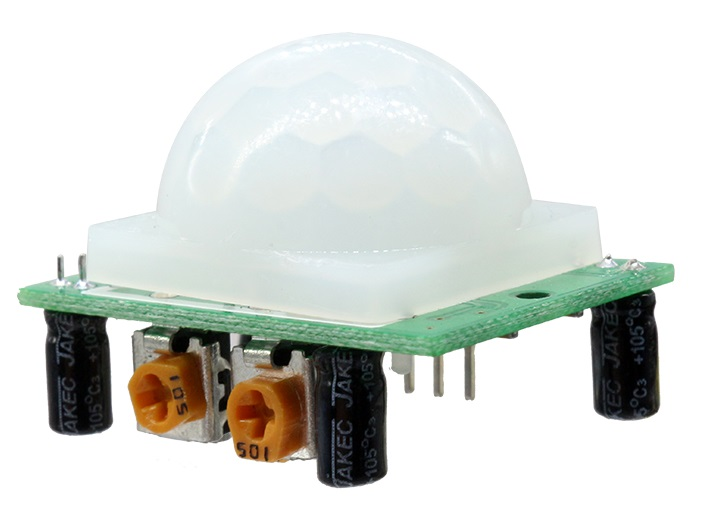
\includegraphics[width=0.3\textwidth]{images/PIR.jpg}
\caption{Detektor pohybu (PIR detektor)}
\label{image}
\end{center}
\end{figure}

\subsection{Komunikátor}
Požadavek na komunikátor je přenos dat do počítače a přes mobilní data. Zadání jako hlavní komunikátor určuje mobilní telefon, pomocí kterého máme umožnit ústředně datové přenosy. Zvolen byl nový a zároveň nejlevnější mobilní telefon na trhu. Pro případ neúspěchu, při získávání zdrojů mobilního telefonu, byla zvolena alternativa v podobě GSM/GPRS modulu, který byl zakoupen z Číny, dodací doba této součástky, stejně jako na všechny ostatní, byla přes jeden kalendářní měsíc.

\paragraph{Zvolené komunikátory:}
\begin{itemize}
\item Mobilní telefon STK R45i Black (449 Kč s DPH), (\url{alza.cz})
\item GSM/GPRS modul (290 Kč s DPH), (\url{aliexpress.com})
\end{itemize} 

\begin{figure}[H]
\begin{center}
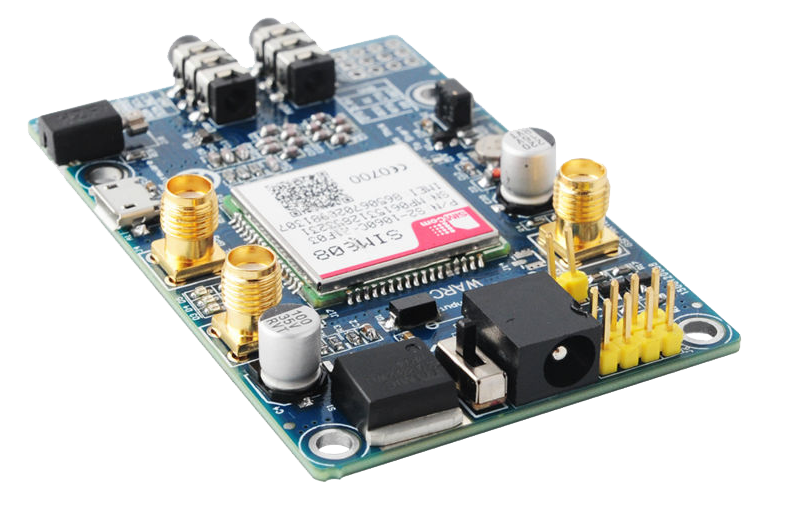
\includegraphics[width=0.5\textwidth]{images/gprs.png}
\caption{Komunikační modul GSM/GPRS - SIM808}
\label{image}
\end{center}
\end{figure}

\section{Software (Ovladač)}
Výše zmíněné prvky musí  být řízeny ovladačem, v mém případě aplikací jak desktopovou tak mobilní. Proto bude následující část rozdělena do těchto dvou částí.

\subsection{Desktopová aplikace}
Na desktopovou aplikaci jsou kladeny požadavky tak, aby byla schopna využít všech možností, které nám ústředna poskytuje. Musí být schopna kompletní správy a nastavení jednotlivých komponent (spínače a senzory) a tím pádem i komunikaci s ní. Cílový operační systém jsem si zvolil Windows 10, jakožto ve škole nejrozšířenější, programovací jazyk C\# a vývojové prostředí Visual Studio 2017. Jednotlivé požadavky kladené na desktopovou aplikaci lze nalézt níže.

\paragraph{Požadavky na desktopovou aplikaci:}
\begin{itemize}
\item Sledování aktuálních stavů komponent
\item Přidávání nových komponent
\item Odstraňování stávajících komponent
\item Přejmenování komponent
\item Změna pinů komponent
\item Změna nastavení senzorů jako spínacích či rozpínacích
\item Notifikace v případě změny stavů senzorů
\item Přepínání stavů spínačů
\item Připojování a odpojování ke zvolené ústředně
\end{itemize} 

\subsection{Mobilní aplikace}
Mobilní aplikace je učena pouze jako monitorovací zařízení, ze kterého bude možné sledovat stavy jednotlivých senzorů, případně spínač spínače. Její návrh je tedy značně jednodušší oproti komplexnější desktopové aplikaci. Cílový operační systém jsem zvolil Android, jakožto nerozšířenější, programovací jazyk Java a vývojové prostředí a Android Studio.

\paragraph{Požadavky na mobilní aplikaci:}
\begin{itemize}
\item Sledování aktuálních stavů komponent
\item Přepínání stavů spínačů
\item Připojování a odpojování ke zvolené ústředně
\end{itemize} 

% Domovní systém (hardware a firmware)

\chapter{Domovní systém}

\section{Využití mobilního telefonu}
Následující část pojednává o snaze využít GSM/GPRS modulu integrovaném v mobilním telefonu. Práce na této části zabrali přibližně dva měsíce, proto bude rozdělena do více částí.

\subsection{Možné postupy}
První úkolem bylo, jak by bylo možné tyto zdroje z mobilního telefonu získat. Průzkumem existujících prací a internetu jsem mohl tento problém rozdělit na dvě kategorie. Chytré telefony a klasické telefony. U chytrých telefonů není získání těchto zdrojů problém, stačí napsat software, který tyto zdroje poskytne přes port USB a tím je problém vyřešen. Klasické telefony se dělí do dvou podkategorií. Telefony s dokumentací s API a poté telefon bez API a dokumentace. Některé starší telefony měli otevřené dokumentace a některá dokonce i API přímo pro tyto účely (Motorola, Nokia), pro tyto mobilní telefony existuje internet plný návodů, jak se dostat ke zdrojům které chceme, nicméně takových modelů je opravdu malé množství. Poslední kategorií jsou mobilní telefony bez otevřených dokumentací a bez API, která by zpřístupňovala chtěné zdroje mobilního telefonu. Pro tyto mobilní telefony jsem nenalezl žádné dostupné řešení, přitom jsou to telefony nejrozšířenější a tím se staly pro tento projekt zajímavými.

\paragraph{Varianty telefonů:}
\begin{itemize}
\item Chytrý telefon (vyřešeno)
\item Klasický telefon s API (vyřešeno)
\item Klasický telefon bez API a dokumentace (nevyřešeno)
\end{itemize} 

\subsection{Výběr telefonu}
Prvním úkolem bylo vybrání vhodného kandidáta pro tyto účely. Bylo tedy nutné zvolit telefon, pro který zatím není problém vyřešen. Po provedení průzkumu trhu jsem zjistil, že je možné vybírat jak z bazarových kousků, tak z nových. Zajímavým zjištěním bylo, že ceny nových telefonů podporujících s funkcí GSM i GPRS startují na 450 Kč s DPH za kus. Bazarové kousky začínají na 600 Kč s DPH za kus. Vzhledem k nižší ceně, záruce a garanci funkčnosti bylo rozhodnuto pro nový kus.

\subsection{První rozbor}
Před obdržením zakoupeného telefonu jsem provedl průzkum, zda existují dokumentace, nebo zda se někdo pokoušel alespoň o něco podobného. Výsledkem bylo, že kromě oficiálního letáku s velice obecnými parametry přístroje, neexistují žádné veřejné dokumentace ani studie zařízení. Ihned po obdržení jsem se tedy pustil do vlastního průzkumu.

\begin{figure}[H]
\begin{center}
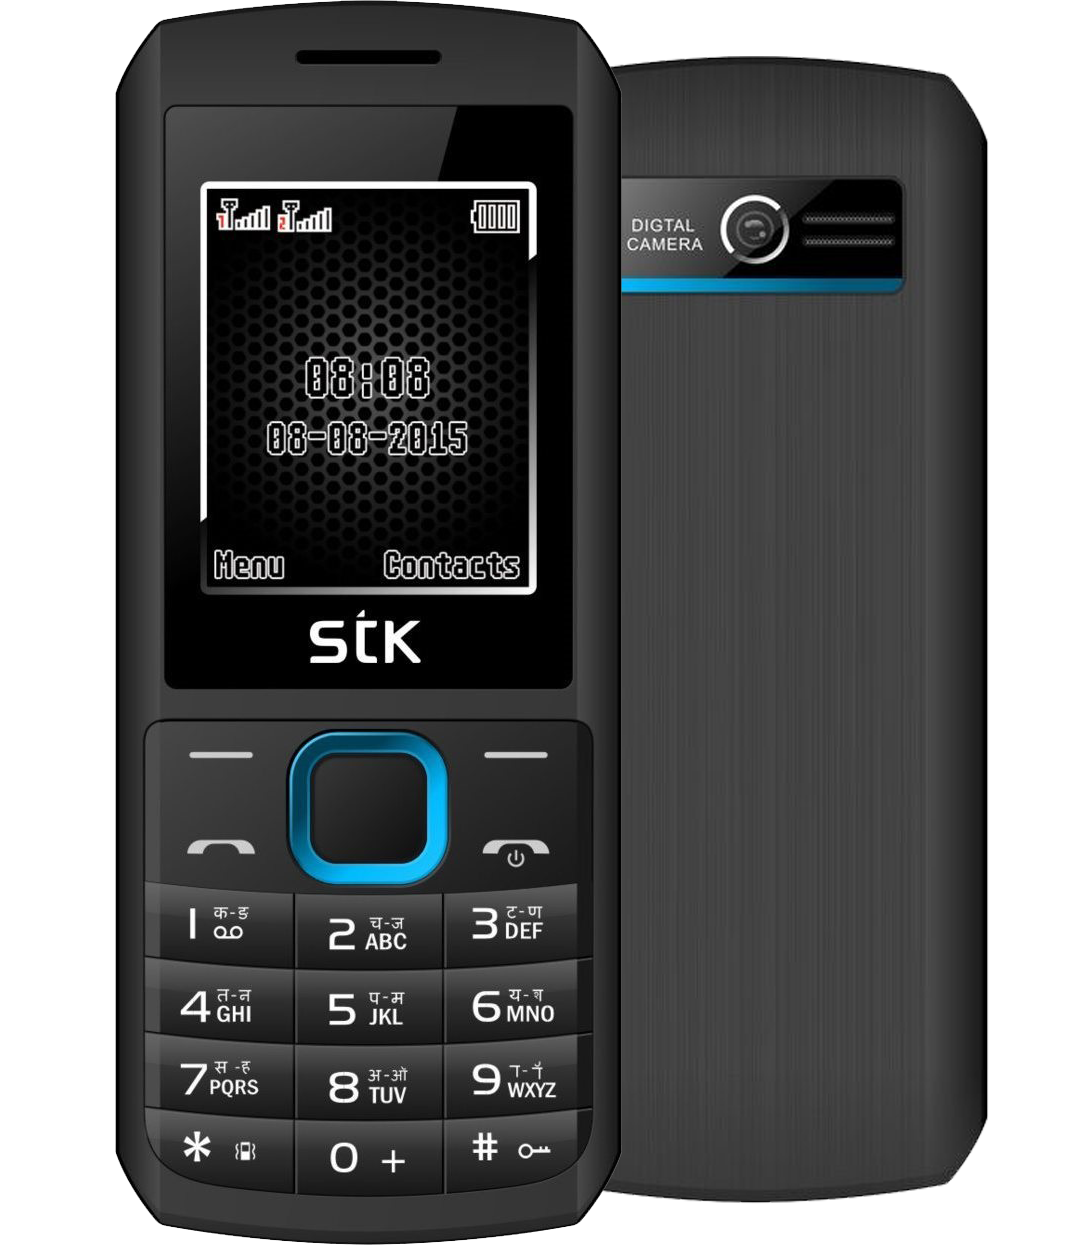
\includegraphics[width=0.4\textwidth]{images/phone.png}
\caption{Zakoupený mobilní telefon}
\label{image}
\end{center}
\end{figure}

\subsection{Kontaktování výrobce}
Jedním z prvních kroků bylo kontaktování výrobce s vysvětlením mého projektu a žádostí o poskytnutí dokumentačních podkladů. Napsal jsem celkem na 3 oddělení britské společnosti, přesněji na obchodní, podporu a servis. Mezitím jsem se pokusil o komunikaci s mobilním telefonem skrze USB, stejně jako to bylo možné u telefonů s API k těmto účelům, to se nepodařilo. Nakonec přišla shodná odpověď ze všech tří kontaktovaných oddělení, tedy že mi dokumentace neposkytnou.

\begin{figure}[H]
\begin{center}

\includegraphics[width=0.6\textwidth]{images/response.png}
\caption{Odpověď od společnosti STK}
\label{image}
\end{center}
\end{figure}

\subsection{Hlubší rozbor}
Bez dokumentací jsem musel začít zkoumat více do hloubky. Po konzultaci s vedoucím byl telefon rozebrán a zkoumán na případné servisní piny pro připojení a diagnostiku. Po hlubším prozkoumání se mi jako jednu variantu podařilo nalézt servisní piny, které jsem se následně snažil analyzovat a skrze ně komunikovat s mobilním telefonem.

\begin{figure}[H]
\begin{center}
\includegraphics[width=0.7\textwidth]{images/servicePins.png}
\caption{Objevené servisní piny}
\label{image}
\end{center}
\end{figure}

\subsection{Závěr rozboru}
Ani po několika týdenním snažení se nepodařilo z pinů dostat žádnou informaci. První týden se mi podařilo zachytávat neznámé signály, nicméně po hlubším přezkoumání spektrálním  analyzátorem bylo zjištěno, že se nejedná o číslicový signál. Po dvouměsíčním zkoumání jsem musel celou věc uzavřít a oznámit vedoucímu, že tudy zřejmě cesta nevede. Od využití mobilního telefonu bylo tedy upuštěno.

\section{Zapojení}

\subsection{Blokové schéma}

\begin{figure}[H]
\begin{center}
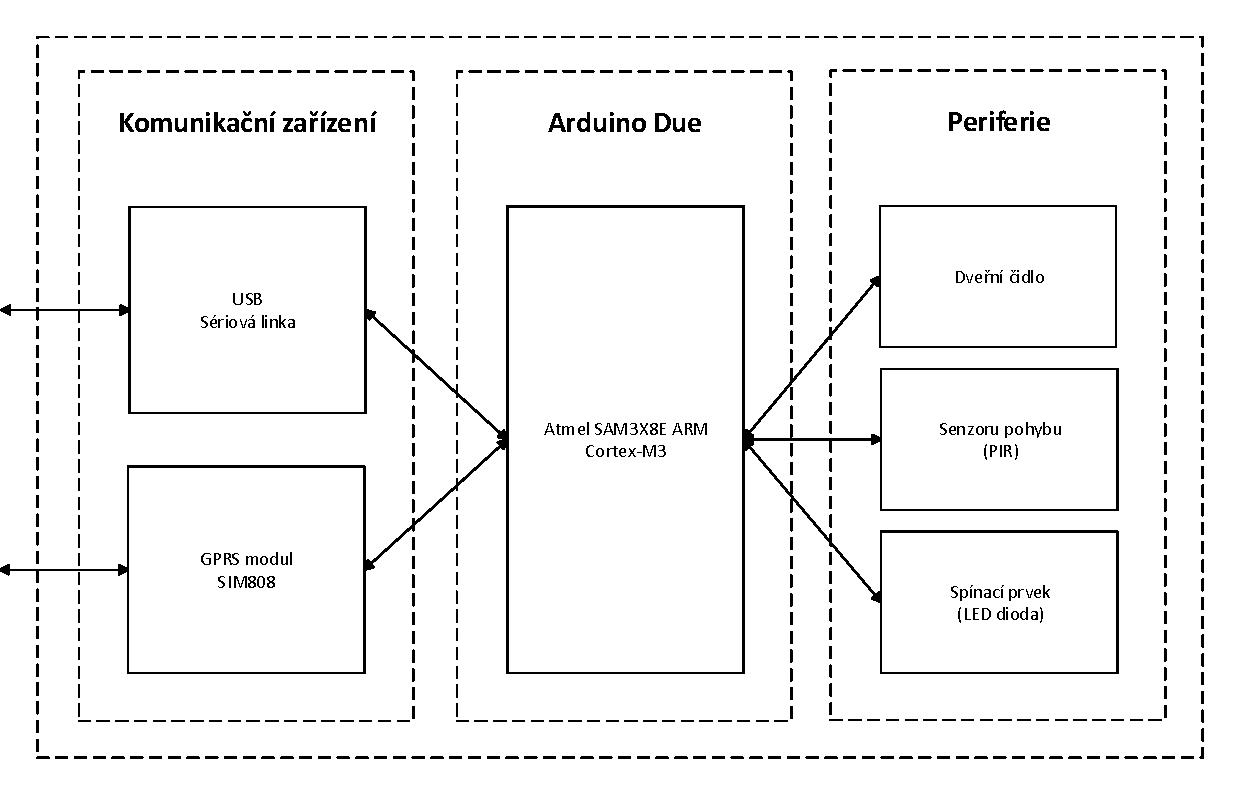
\includegraphics[width=\textwidth]{vector/blokoveSchemaHardware.pdf}
\caption{Blokové schéma zapojení prototypu zabezpečovacího zařízení}
\label{image}
\end{center}
\end{figure}

\subsection{Výsledný prototyp}
Výsledný prototyp je schopen simulovat reálné nasazení zabezpečovacího systému. Obsahuje (zleva) řídící desku Arduino, jednu diody (LED) pro simulování spínacího prvku, dále diodu která signalizuje, zda je sepnutý senzor PIR, a diodu signalizující sepnutí dveřního čidla (vpravo). 

\begin{figure}[H]
\begin{center}
\includegraphics[width=\textwidth]{images/board.png}
\caption{Finální prototyp na nepájivém poli}
\label{image}
\end{center}
\end{figure}

\section{Firmware}
Hlavním účelem firmwaru je možnost kompletního řízení zabezpečovacího systému a umožnění komunikace, včetně poskytování API pro přístup aplikací. Software byl vyvinut pro platformu Arduino (čip ATmega) v programovacím jazyce C++ s nadstavbou Wiring (knihovna pro řízení hardwaru) \cite{Wiring}, za pomocí vývojového prostředí Visual Studio 2017 s rozšířením Visual Micro \cite{Visual Micro}, které poskytuje zvýrazňování syntaxe knihovny Wiring a umožňuje komplikaci a nahrávání kódu přímo na desku Arduino.

Dále budou zmíněny pouze ty části, které jsou důležité pro pochopení nastavení zařízení a přístupu k aplikaci (API), samotný kód lze nalézt v příloze a zmiňován zde nebude.

\subsection{Nastavení}
Inicializační část slouží k prvotnímu nastavení mikrokontroleru před spuštěním. Toto nastavení po nahrání kódu do zařízení nelze měnit. Jedinou cestou k jeho změně je tedy opětovná kompilace kódu s upraveným nastavením a následné nahrání do mikrokontroleru.

\paragraph{Nastavit lze:}
\begin{itemize}
\item Komunikační rychlost (baudRate)
\item Maximální počet senzorů
\item Maximální počet spínačů
\item Kódy chybových hlášek
\item Klíčová slova API
\end{itemize} 

\subsection{API}
Funkce API jsou nazvány podle své činnosti. Při volání jednolivých funkcí se posílá nejdříve název funkce, které následují kulaté závorky, tedy \uv{(} a \uv{)}, vnichž jsou uvedeny jednotlivé parametry. Každý jeden parametr je oddělen čárkou. Ve výsledku může výstup vypadat například takto \uv{SetSensor(10,5)}. V následující tabulce jsou vypsány všechny dostupné funkce, typu getter.

\renewcommand{\arraystretch}{1.5}
\begin{table}[H]
\begin{center}
\begin{tabular}{| l | c | c| c |}
\hline
Funkce & Parametry & Popis & Vrací\\
\hline
\hline
GetAllSensors() & / & Vrací list všech senzorů & id, pin, name, state \\
\hline
GetAllSwitches() & / & Vrací list všech spínačů & id, pin, name, state \\
\hline
\end{tabular}
\end{center}
\caption{Tabulka API - Getters}
\end{table}

\paragraph{Ukázka vrácených senzorů:}
\begin{center}
Sensors((Id = 0,Pin = 8,Name = Door Sensor,State = 0,Type = 0)(Id = 1,Pin = 7,Name = PIR Sensor,State = 0,Type = 1))
\end{center} 

\paragraph{Ukázka vrácených spínačů:}
\begin{center}
Switches((Id = 0,Pin = 6,Name = Led Switch,State = 0))
\end{center} 

Další tabulka obsahuje výpis všech dostupných funkcí, typu setter.

\renewcommand{\arraystretch}{1.5}
\begin{table}[H]
\begin{center}
\begin{tabular}{| l | c | c| c |}
\hline
Dotaz & Parametry & Popis & Vrací\\
\hline
\hline
SetSensorName() & id, name & Změna jména senzoru & OK, ERROR \\
\hline
SetSwitchName() & id, name & Změna jména spínače & OK, ERROR \\
\hline
SetSensorPin() & id, pin & Změna pinu senzoru & OK, ERROR \\
\hline
SetSwitchPin() & id, pin & Změna pinu spínače & OK, ERROR \\
\hline
SetSensorType() & id, type & Změna typu senzoru & OK, ERROR \\
\hline
SetSwitchState() & id, state & Změna stavu spínače & OK, ERROR \\
\hline
AddSensor() & pin, name, type & Přidání nového senzoru & OK, ERROR \\
\hline
AddSwitch() & pin, name, state & Přidání nového spínače & OK, ERROR \\
\hline
DeleteSensor() & id & Smazání senzoru & OK, ERROR \\
\hline
DeleteSwitch() & id & Smazání spínače & OK, ERROR \\
\hline
\end{tabular}
\end{center}
\caption{Tabulka API - Setters}
\end{table}

U nastavovacích dotazů musí být \uv{id} a \uv{pin} číslo od 0 do 100, \uv{type} a \uv{state} musí být číselné hodnoty 0 (false) nebo 1 (true) a \uv{name} musí být maximálně 30 znaků dlouhé (30 bytů). Pro \uv{state} znamená 1 zapnuto, 0 vypnuto. Pro \uv{type} znamená 1 \uv{normálně vypnuto / push to make} a 0 \uv{normálně zapnuto / push to break}. Pokud jedna z podmínek nebude splněna, dotaz bude odmítnut. Parametr \uv{ID} lze získat pomocí příkazu \uv{GetAllSensors()} a \uv{GetAllSwitches} z již existujících zařízení.

\paragraph{Ukázka přidání nového senzoru:}
\begin{center}
AddSensor(8, Muj novy senzor, 0)
\end{center}

\paragraph{Ukázka změny pinu senzoru:}
\begin{center}
SetSensorName(1, Moje nove jmeno senzoru)
\end{center}

\paragraph{Ukázka smazání spínače:}
\begin{center}
DeleteSwitch(1)
\end{center}

\subsection{Notifikace}
Bezpečnostní zařízení má uložené všechny poslední stavy senzorů a při každém průchodu hlavní smyčkou proběhne čtení, pomocí funkce \uv{checkSensorStateChangedAndSendIfTrue()}. Pokud nový stav nesouhlasí se starým, je zaslána notifikace s ID zařízení a aktuálním stavem. Poté záleží na cílové aplikaci, jak informaci zpracuje.

\paragraph{Ukázka notifikace:}
\begin{center}
Sensor(Id = 1,State = 0)
\end{center} 

\subsection{Chybová hlášení}
Původně byla chybová hlášení (při neúspěšném provedení operace nebo jiné chybě), tvořena pomocí stavových kódů HTML \cite{HTML1.1}. Z důvodu nedostatku paměti byla nahrazena jednoduchým \uv{OK} a \uv{ERROR}. Kontrola chyb se provádí vždy při provádění kterékoliv z operací podporující API. Vždy se kontroluje, zda je možné zapsat, zda se provedl zápis, zda je nová hodnota po přečtení stejná jako zapisovaná, a tak dále. Pokud nastane chyba, je vše vráceno do původního stavu. Pokud příkaz nebyl rozpoznán, nebo nesplňuje kritéria tohoto API, je vrácena chybová hláška o nerozpoznání příkazu.
\paragraph{Ukázka odpovědi při nerozpoznání příkazu:}
\begin{center}
Command 'SetSensor(15,5)' not recognized.
\end{center} 

% Desktopová aplikace

\chapter{Desktopová aplikace}
Hlavním účelem desktopové aplikace je možnost kompletního nastavení a monitorování zabezpečovacího zařízení. Aplikace se zaměřuje zejména na správu (vytváření, upravování, mazání) všech senzorů a spínačů. Software byl vyvinut pro operační systém Windows v programovacím jazyce C\#, za pomocí IDE Visual Studio 2017.

\section{Kompatibilita}
Desktopová aplikace byla testována pod operačním systémem Windows 10 ve všech (v době psaní práce) vydaných sestavách a pro tento systém byla také optimalizována. Nicméně cílová platforma Microsoft .NET Framework 4.5.2 \cite{WhatsNew.NetFramework4.5.2} by měla zajišťovat zpětnou kompatibilitu až do systému Windows Vista. Jmenovitě pro Windows Vista SP2, Windows 7 SP1, Windows 8, Windows 8.1, Windows 10 a novější \cite{.NetFramework4.5.2}.

\paragraph{Seznam všech testovaných sestav systému Windows 10:}
\begin{itemize}
\item Version 1507 - Build 10.0.10240 (čistá instalace systému)
\item Version 1511 - Build 10.0.10586 (November Update)
\item Version 1607 - Build 10.0.14393 (Anniversary Update)
\item Version 1703 - Build 10.0.15063 (Creators Update)
\item Version 1709 - Build 10.0.16299 (Fall Creators Update)
\end{itemize}

\section{Blokové schéma}

\begin{figure}[H]
\begin{center}
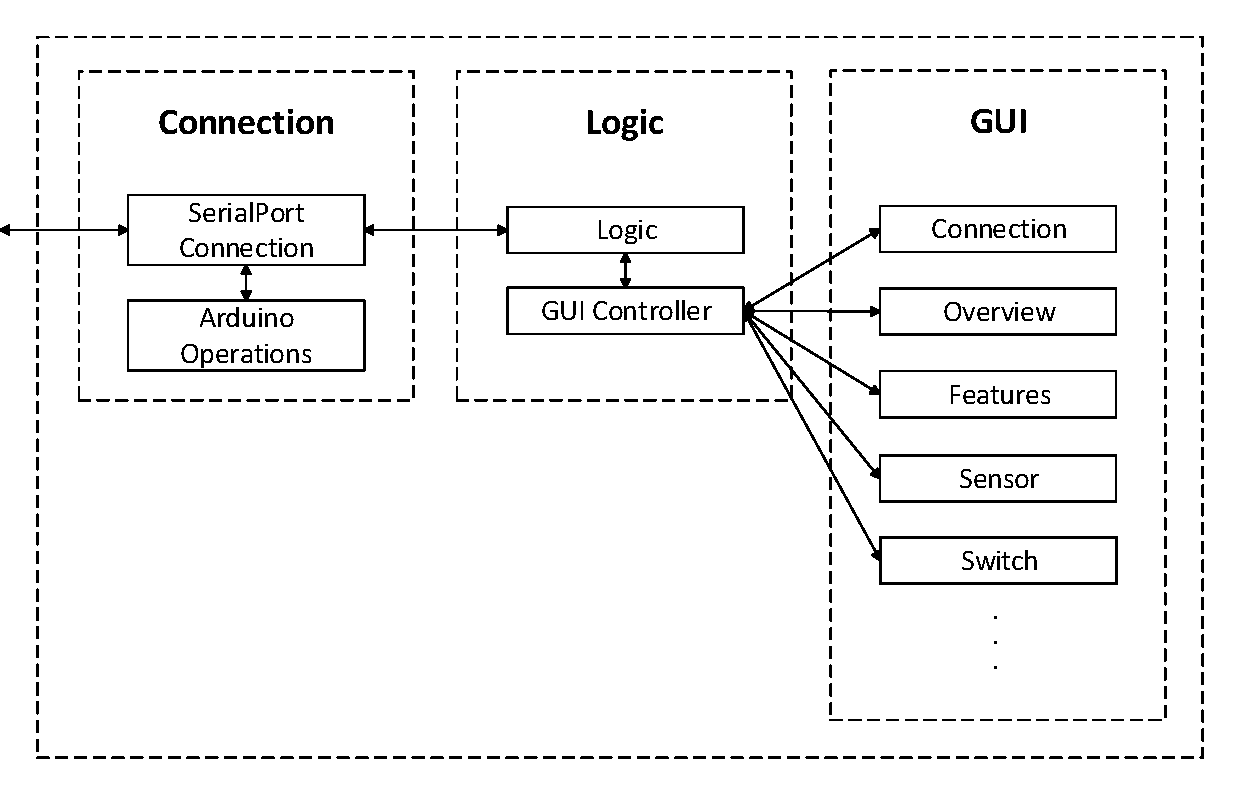
\includegraphics[width=\textwidth]{vector/blokoveSchemaSecurityControl.pdf}
\caption{Blokové schéma objektového návrhu aplikace}
\label{image}
\end{center}
\end{figure}

Kód aplikace je rozdělen do více spolu bloků, které spolu vzájemně komunikují. Arduino Connector slouží k napojení zabezpečovacího zařízení a využívá API poskytované zabezpečovacím zařízením, díky čemuž poskytuje funkce pro jednoduché zapisování a čtení do Arduina. Windows Forms poskytují grafické uživatelské rozhraní, základní logiku na propojení jednotlivých funkčních celků a notifikace pro uživatele. UserControls poskytují jednotlivé funkce aplikace, z nichž každá má své vlastní GUI, které se zobrazuje ve Windows Forms. Dále budou zmíněny pouze ty UserContorls, které jsou důležité pro pochopení ovládání aplikace. Design byl inspirovaný manuálem jednotného vizuálního stylu TUL \cite{TULVisual}.

\section{Spojení}

\begin{figure}[H]
\begin{center}
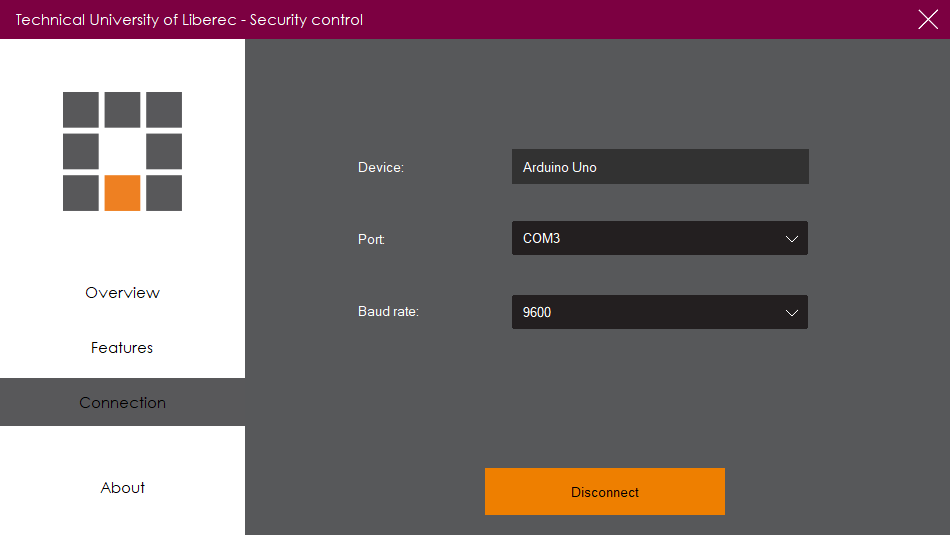
\includegraphics[width=\textwidth]{images/connection.png}
\caption{Okno s možností připojení/odpojení od řídící jednotky}
\label{image}
\end{center}
\end{figure}

Spojení slouží k připojení či odpojení od zabezpečovacího zařízení. Za běhu aplikace na pozadí hlídá, zda je připojení stále navázáno. Při ztrátě spojení ihned informuje uživatele a upraví chování celé aplikace. Spojení rovněž hlídá, zda se neobjevilo nové zařízení k připojení, pokud ano, informuje uživatele a zobrazí nově dostupná zařízení.

\section{Přehled}

\begin{figure}[H]
\begin{center}
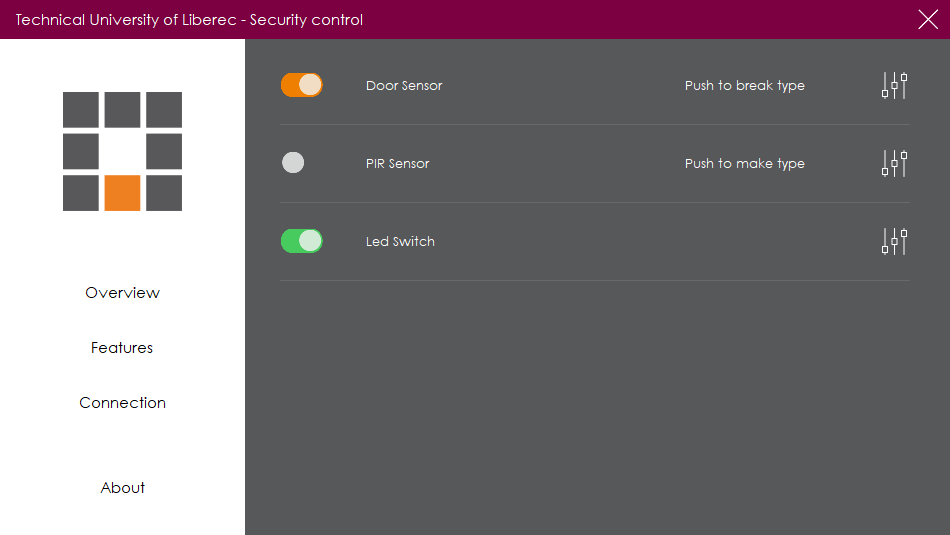
\includegraphics[width=\textwidth]{images/overview.png}
\caption{Okno s přehledem jednotlivých komponent}
\label{image}
\end{center}
\end{figure}

Přehled slouží pro zobrazení všech dostupných spínačů a senzorů, které jsou v zabezpečovacím zařízení dostupné. Obsah se generuje dynamicky pod sebe, lze tedy vytvořit neomezený počet zobrazených zařízení. Každý dynamický řádek je zobrazen dle svého typu, tedy zda se jedná o senzor nebo spínač. U spínačů lze měnit jejich aktuální stav, u senzorů lze aktuální stav pouze sledovat. V obou případech lze měnit interní nastavení každého zařízení, pomocí tlačítka na pravé straně. V případě, že žádná zařízení neexistují, je uživatel upozorněn. Žádná data nejsou měněna v objektech uvnitř aplikace, ale změny jsou poslány do zabezpečovacího zařízení, po obdržení odpovědi se změní stav v aplikaci a uživatel je upozorněn.

\section{Nastavení senzoru}

\begin{figure}[H]
\begin{center}

\includegraphics[width=\textwidth]{images/settings.png}
\caption{Okno s nastavením komponenty (Senzor)}
\label{image}
\end{center}
\end{figure}

Nastavení senzoru slouží k změně interního nastavení uvnitř zabezpečovacího zařízení. Lze měnit název zařízení, pin na kterém se nachází a typ tohoto zařízení (rozpínací, spínací). Výběr pinů závisí vždy na připojené desce, pro tento účel byl vytvořen kompletní seznam desek Arduino (USA) a Genuino (Evropa), dnes již znovu pouze Arduino, s kompletním seznamem pinů, které lze použít. Poslední funkcí je smazání zařízení.

\section{Nastavení spínače}
Nastavení je téměř identické s předchozím, lze měnit název, pin, a místo typu zařízení lze přenastavit jeho stav.

\section{Funkce programu a nastavení}
Tato záložka zpřístupňuje různá nastavení a funkce, které nejsou běžně potřebné.

\paragraph{Přehled funkcí:}
\begin{itemize}
\item Přidat nový senzor
\item Přidat nový spínač
\item Znovu načíst všechna data ze zabezpečovacího zařízení
\item Zobrazovat notifikace, pokud se změní stav senzoru (přepínač)
\item Zobrazovat notifikace, pokud se senzor navrátí do výchozího stavu (přepínač)
\end{itemize} 

\section{Notifikace}
Aplikace podporuje širokou škálu notifikací, upozornění a varovných hlášení, která slouží při upozornění uživatele na nějakou situaci. Například se jedná o změnu stavu pinů, chybové stavy řídící jednotky, nebo odpojení zabezpečovacího zařízení. Notifikace se zachytávají v hlavním okně, v záložce \uv{Autocalled functions (Events from Arduino)}, pomocí eventů.

\paragraph{Přehled implementovaných notifikací:}
\begin{itemize}
\item Připojení zabezpečovacího zařízení
\item Odpojení zabezpečovacího zařízení
\item Ztráta spojení zabezpečovacího zařízení
\item Automatický pokus o připojení se nezdařil
\item Stav spínače přenastaven
\item Stav senzoru se změnil
\item Interní chyba řídící jednotky
\item Jméno se podařilo/nepodařilo změnit
\item PIN se podařilo/nepodařilo změnit
\item Typ senzoru se podařilo/nepodařilo změnit
\item Nový senzor se podařilo/nepodařilo přidat
\item Nový spínač se podařilo/nepodařilo přidat
\item Komponenty arduina se podařilo/nepodařilo znovu načíst
\item Nastavení notifikací změněno
\end{itemize} 

% Komunikační server

\chapter{Komunikační server}
Not implemented yet.

% Mobilní aplikace

\chapter{Mobilní aplikace}
Hlavním účelem mobilní aplikace je monitorování zabezpečovacího zařízení, a není tedy možno měnit jakékoliv nastavení, k čemuž slouží desktopová aplikace. Aplikace byla vyvinuta pro mobilní operační systém Android 4.0.3 (Ice Cream Sandwich - API 15) a vyšší, v programovacím jazyce Java, za pomocí IDE Android Studio 2.3.2.

\section{Přehled}
\begin{figure}[H]
\begin{center}
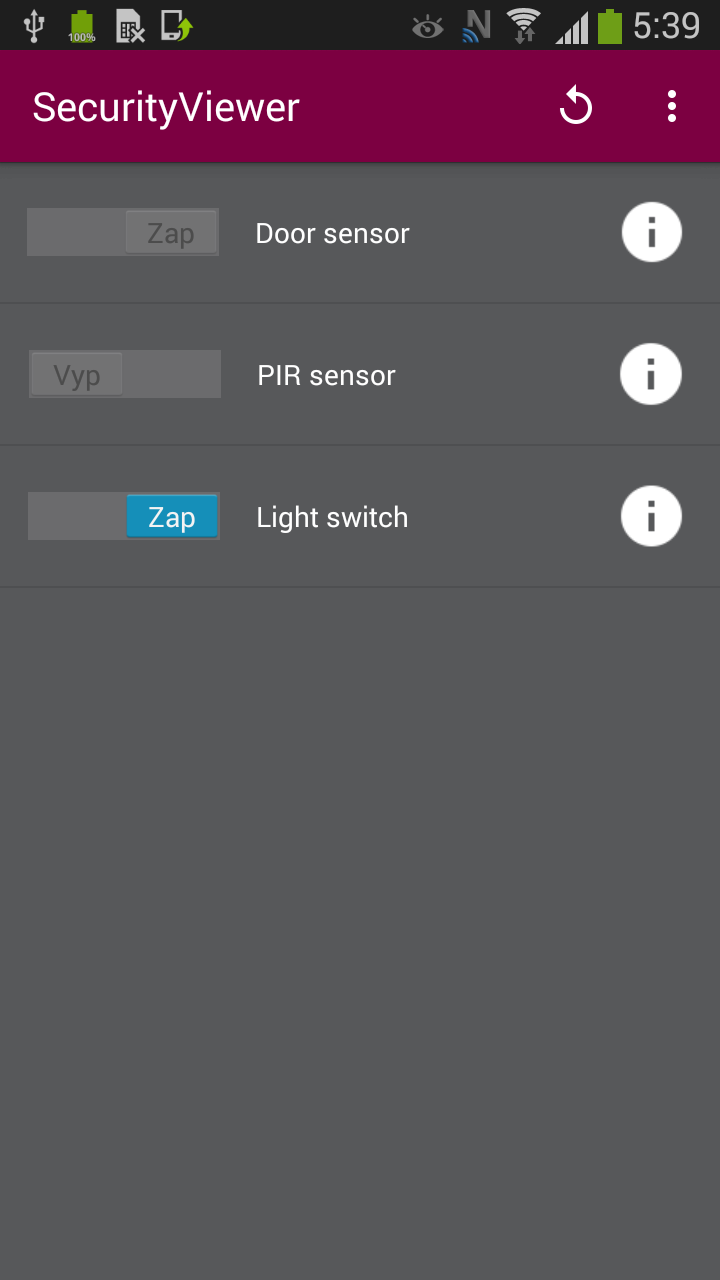
\includegraphics[width=0.4\textwidth]{images/app1.png}
\caption{Okno s přehledem jednotlivých komponent}
\label{image}
\end{center}
\end{figure}

Stejně jako v případě desktopové aplikace, slouží přehled pro zobrazení všech dostupných spínačů a senzorů, které jsou v zabezpečovacím zařízení dostupné. Obsah se generuje dynamicky pod sebe, lze tedy vytvořit neomezený počet zobrazených zařízení. Každý dynamický řádek je zobrazen dle svého typu, tedy zda se jedná o senzor nebo spínač. U spínačů lze měnit jejich aktuální stav, u senzorů lze aktuální stav pouze sledovat. V obou případech lze zobrazit interní nastavení každého zařízení, pomocí tlačítka na pravé straně. Žádná data nejsou měněna v objektech uvnitř aplikace, ale změny jsou poslány do zabezpečovacího zařízení, po obdržení odpovědi se změní stav v aplikaci a uživatel je upozorněn.

\section{Interní nastavení}
\begin{figure}[H]
\begin{center}
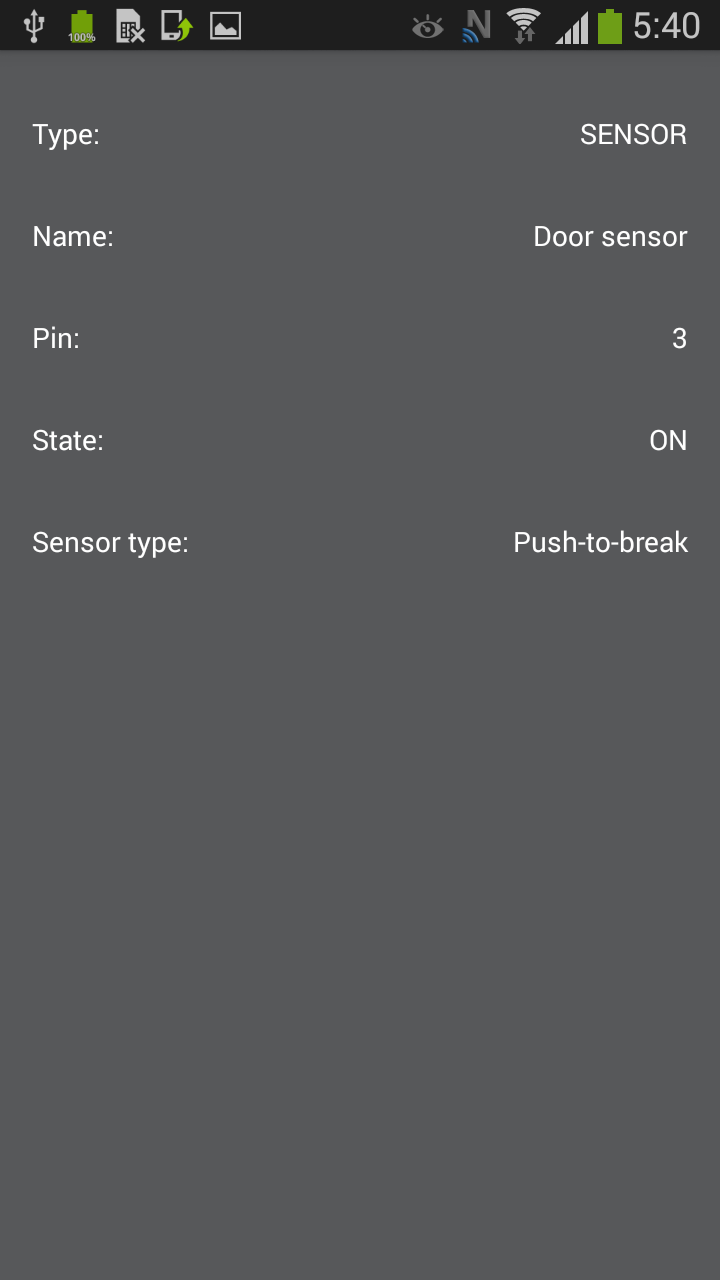
\includegraphics[width=0.4\textwidth]{images/app2.png}
\caption{Detailní přehled nastavení komponenty}
\label{image}
\end{center}
\end{figure}

Zobrazení interního nastavení jednotlivých komponent ukazuje méně důležité údaje. Vrátit se lze tlačítkem zpět, které má každý mobilní telefon se systémem Android implementované (ať už softwarově nebo hardwarově).

% Webová aplikace

\chapter{Webová aplikace}
Not implemented yet.

% Závěr

\chapter{Závěr}
Not implemented yet.

% Literatura

\addcontentsline{toc}{chapter}{Literatura}
\begin{thebibliography}{10}
\bibitem{Bachelor thesis}MORAVEC, Tomáš. Koncept nízkonákladového sledovacího zařízení pro osobní automobily: The concept of a low cost tracking device for personal cars. Liberec: Technická univerzita v Liberci, 2016.
\bibitem{Security alarm}Security alarm. Wikipedia [online]. [cit. 2017-05-23]. Dostupné z: \url{https://en.wikipedia.org/wiki/Security_alarm}
\bibitem{Electronic security system}Elektronické zabezpečovací systémy [online]. , 1 [cit. 2017-05-23]. Dostupné z: \url{http://www.ezasys.cz/elektronicke-zabezpecovaci-systemy/}
\bibitem{Electronic security signalisation}Elektronická zabezpečovací signalizace. Wikipedia [online]. [cit. 2017-05-23]. Dostupné z: \url{https://cs.wikipedia.org/wiki/Elektronick\%C3\%A1\_zabezpe\%C4\%8Dovac\%C3\%AD_signalizace}
\bibitem{Wiring}Wiring [online]. [cit. 2016-05-08]. Dostupné z: \url{http://wiring.org.co/}
\bibitem{Visual Micro}Visual Micro [online]. [cit. 2017-05-23]. Dostupné z: \url{http://www.visualmicro.com/}
\bibitem{Arduino intro}Arduino introduction. Arduino [online]. [cit. 2017-05-23]. Dostupné z: \url{https://www.arduino.cc/en/Guide/Introduction}
\bibitem{Arduino lib}Arduino libraries. Arduino [online]. [cit. 2016-05-08]. Dostupné z: \url{https://www.arduino.cc/en/Reference/Libraries}
\bibitem{Arduino lang}Arduino programming language. Arduino [online]. [cit. 2016-05-08]. Dostupné z: \url{https://www.arduino.cc/en/Reference/HomePage}
\bibitem{Arduino schematic}ARDUINO LLC. Arduino Schematic [online]. 1 s. [cit. 2016-05-07]. Dostupné z: \url{https://www.arduino.cc/en/uploads/Main/Arduino\_Uno\_Rev3-schematic.pdf}
\bibitem{Arduino soft} Arduino software. Arduino [online]. [cit. 2016-05-08]. Dostupné z: \url{https://www.arduino.cc/en/Main/Software}
\bibitem{Arduino source}Arduino source code. GitHub [online]. [cit. 2016-05-08]. Dostupné z: \url{https://github.com/arduino/Arduino/tree/1.6.8}
\bibitem{Atmega datasheet}ATMEL CORPORATION. ATmega48A/PA/88A/PA/168A/PA/328/P Datasheet [online]. 2015, 660 s. [cit. 2016-05-07]. Dostupné z: http://www.atmel.com/images/Atmel-8271-8-bit-AVR-Microcontroller-ATmega48A-48PA-88A-88PA-168A-168PA-328-328P\_ datasheet\_Complete.pdf
\bibitem{LaTeX}SATRAPA, Pavel. LaTeX pro pragmatiky [online]. 2011, 87 s. [cit. 2016-05-07]. Dostupné z: \url{http://www.nti.tul.cz/~satrapa/docs/latex/latex-pro-pragmatiky.pdf}
\bibitem{Pruvodce arduinem}VODA, Zbyšek. Průvodce světem Arduina [online]. Vydání první. Bučovice: Martin Stříž, 2015 [cit. 2016-05-07]. ISBN 978-80-87106-90-7.
\bibitem{SIMCOM SW}SIMCOM WIRELESS SOLUTIONS. SIM908 AT Command Manual [online]. Jinzhong, 2011, 249 s. [cit. 2016-05-07]. Dostupné z: \url{http://www.dfrobot.com/image/data/TEL0051/3.0/SIM908\_AT\%20Command\%20Manua\_V1.01.pdf}
\bibitem{SIMCOM HW}SIMCOM WIRELESS SOLUTIONS. SIM908 Hardware Design [online]. 2. Jinzhong, 2012, 53 s. [cit. 2016-05-07]. Dostupné z: \url{http://www.niplesoft.net/blog/wp-content/uploads/2016/02/SIM908-Hardware-Design-V2.00-1.pdf}
\bibitem{LaTeX}SATRAPA, Pavel. Stručný přehled příkazů LaTeXu [online]. 2011, 2 s. [cit. 2016-05-07]. Dostupné z: \url{http://www.nti.tul.cz/~satrapa/docs/latex/latex-prehled.pdf}
\bibitem{TULVisual}Manuál jednotného vizuálního stylu Technické univerzity v Liberci [online]. , 27 [cit. 2017-05-27]. Dostupné z: \url{http://www.ft.tul.cz/document/126}
\bibitem{HTML1.1}FIELDING, R., UC IRVINE, J. GETTYS, et al. Hypertext Transfer Protocol -- HTTP/1.1 [online]. 1999, , 176 [cit. 2017-05-27]. Dostupné z: \url{http://www.ietf.org/rfc/rfc2616.txt}
\bibitem{WhatsNew.NetFramework4.5.2}What's new in the .NET Framework 4.5.2. Microsoft.com [online]. [cit. 2018-02-21]. Dostupné z: \url{https://docs.microsoft.com/en-us/dotnet/framework/whats-new/index#v452}
\bibitem{.NetFramework4.5.2}Microsoft .NET Framework 4.5.2. Microsoft.com [online]. [cit. 2018-02-21]. Dostupné z: \url{https://support.microsoft.com/en-us/help/2901907/microsoft-net-framework-4-5-2-offline-installer-for-windows-server-201}


\end{thebibliography}

% Příloha

\appendix
\chapter{Obsah přiloženého CD}
Not implemented yet.

\end{document}